\begin{figure}[!htb]
\centering
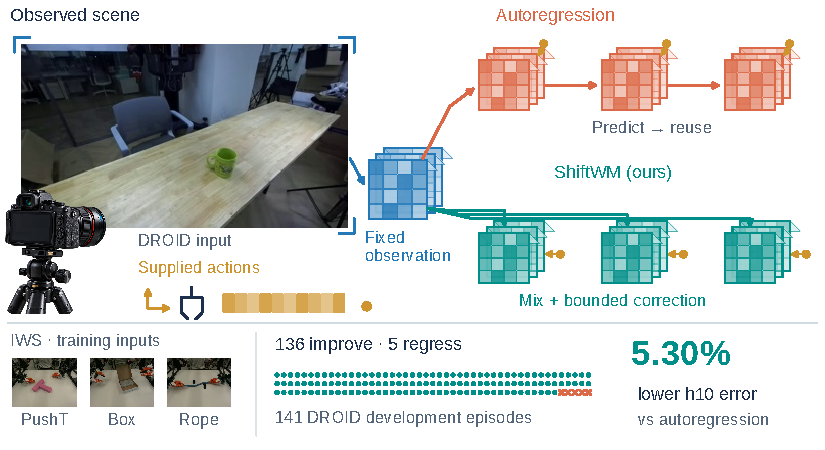
\includegraphics[width=\linewidth]{generated/editorial/teaser_cinematic.pdf}
\caption[Forecast from a fixed observed reference.]{\textbf{Forecast from a fixed observed reference.} The DROID image is the prespecified median episode\textquotesingle s last support frame. Autoregression feeds forecasts forward; ShiftWM mixes fixed observed features and adds bounded corrections. Gold ports denote supplied causal action prefixes; both routes share observed history. Three schematic steps depict the ten-step forecast. The generated foreground camera is illustrative; no predicted RGB or measured error trajectory is shown. Bottom: all 141 development episodes. The 5.30\% reduction compares population mean native, training-standardized h10 feature MSE against matched autoregression, not the mean episode percentage. Uncertainty: Figure~\ref{fig:editorial-spatial}. IWS photos are separate internal-training inputs; training is in progress. Images: DROID (CC BY 4.0) and IWS \citep{zhang2026rlawm}.}
\label{fig:editorial-teaser}
\end{figure}
